\documentclass[a4,paper,fleqn]{article}

\usepackage{layout}

\DeclareSIUnit\year{Jahr}
\newcommand{\wye}{
    \begin{tikzpicture}
        \draw ( 90:0) -- ( 90:0.2);
        \draw (210:0) -- (210:0.2);
        \draw (330:0) -- (330:0.2);
    \end{tikzpicture}
}

\title{Notizen EEV -- SW02}
\date{\today}
\author{Daniel Winz}

\begin{document}
\maketitle
\clearpage

\section{Neutralleiterspannung}
\[ \underline{U}_{KN} =
    \frac{
        \frac{\underline{U}_{1N}}{\underline{Z}_{1}} +
        \frac{\underline{U}_{2N}}{\underline{Z}_{2}} +
        \frac{\underline{U}_{3N}}{\underline{Z}_{3}}
    }
    {
        \frac{1}{\underline{Z}_{1}} +
        \frac{1}{\underline{Z}_{2}} +
        \frac{1}{\underline{Z}_{3}} +
        \frac{1}{\underline{Z}_{N}}
    }
\]
\begin{figure}[h!]
    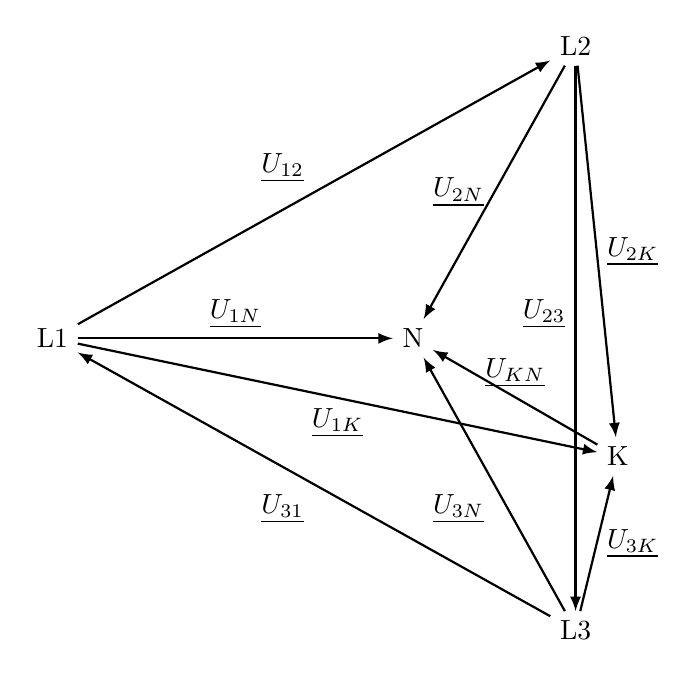
\begin{tikzpicture}
        \node(l1) at (180:4) [left]        {L1};
        \node(l2) at ( 60:4) [above right] {L2};
        \node(l3) at (300:4) [below right] {L3};
        \node(n)  at (  0:0) [right]       {N};
        \node(k)  at (330:3) [right]       {K};
        \draw[thick, -latex] (l1) -- node[above left] {$\underline{U_{12}}$} (l2);
        \draw[thick, -latex] (l2) -- node[above left] {$\underline{U_{23}}$} (l3);
        \draw[thick, -latex] (l3) -- node[below left] {$\underline{U_{31}}$} (l1);
        \draw[thick, -latex] (l1) -- node[above]      {$\underline{U_{1N}}$} (n);
        \draw[thick, -latex] (l2) -- node[left]       {$\underline{U_{2N}}$} (n);
        \draw[thick, -latex] (l3) -- node[below left] {$\underline{U_{3N}}$} (n);
        \draw[thick, -latex] (l1) -- node[below]      {$\underline{U_{1K}}$} (k);
        \draw[thick, -latex] (l2) -- node[right]      {$\underline{U_{2K}}$} (k);
        \draw[thick, -latex] (l3) -- node[right]      {$\underline{U_{3K}}$} (k);
        \draw[thick, -latex] (k)  -- node[above]      {$\underline{U_{KN}}$} (n);
    \end{tikzpicture}
\end{figure}

\section{Vorteile des Drehstroms}
\begin{itemize}
    \item 2 Spannungen verfügbar: \\
        $U_{S}$ und $\sqrt{3} \cdot U_{S} = U$ verkettet
    \item Erzeugung eines Drehfeldes (Drehfeldmaschinen)
    \item Weniger Leitermaterial im Vergleich zur einphasigen Übertragung
    \item Bei symmetrischer Belastung ist die Wirkleistung zeitlich konstant (alle 3 Phasen zusammen)
\end{itemize}

\section{Symmetrische Belastung}
Überall $\underline{Z} = Z \angle\varphi_Z$

\subsection{Sternschaltung (mit oder ohne Neutralleiter)}
\begin{itemize}
    \item Strangspannungen = Phasenspannung
        \[ U_{1K} = U_{2K} = U_{3K} = \frac{U}{\sqrt{3}} = U_S \]
    \item Strangströme = Aussenleiterströme
        \[ I_1 = I_2 = I_3 = \frac{U_S}{Z} = I \]
    \item Scheinleistung
        \[ S = 3 \cdot U_s \cdot I = 3 \cdot \frac{U}{\sqrt{3}} \cdot I = \sqrt{3} \cdot U \cdot I \]
        \[ \boxed{S = \sqrt{3} \cdot U \cdot I \qquad 
            \underline{S} = \sqrt{3} \cdot U \cdot I \angle \varphi_Z} \]
\end{itemize}

\subsection{Dreieckspannung}
\begin{itemize}
    \item Strangspannungen = verkettete Spannungen
        \[ U_{12} = U_{23} = U_{31} = U \]
    \item Strangströme
        \[ I_{12} = I_{23} = I_{31} = \frac{U}{Z} = I_{\triangle} \]
    \item Aussenleiterströme
        \[ I_1 = I_2 = I_3 = \sqrt{3} \cdot I_{\triangle} = I \]
    \item Scheinleistung
        \[ S = 3 \cdot U \cdot I_{\triangle} = 3 \cdot U \cdot \frac{I}{\sqrt{3}} = \sqrt{3} \cdot U \cdot I \]
        \[ \boxed{S = \sqrt{3} \cdot U \cdot I \qquad 
            \underline{S} = \sqrt{3} \cdot U \cdot I \angle \varphi_Z} \]
\end{itemize}

\section{Leistungsvergleich $\star$ - $\triangle$}
\begin{tabular}{ll}
    $\star$:     & $S_{\star} = \dfrac{U^2}{Z}$ \\ 
    $\triangle$: & $S_{\triangle} = 3 \cdot \dfrac{U^2}{Z}$ \\
\end{tabular}
\[ \Rightarrow S_{\triangle} = 3 \cdot S_{\star} \]
\[ \Rightarrow P_{\triangle} = 3 \cdot P_{\star} \]
\[ \Rightarrow Q_{\triangle} = 3 \cdot Q_{\star} \]

\section{Stromverteilung}
UCTE $\stackrel{2009}{\to}$ ENTSO-E (European Network of Transmission System Operators for Electricity

\section{Normwerte}
\subsection{Nennwert (Nominal value)}
Dient zur Benennung einer Grösse \\
Index: $N$ \\
Bsp: $U_N = 380 \si{\kilo\volt}$

\subsection{Bemessungswert (Rated value)}
Beschreibt eine Betriebsbedingung \\
Index: r \\
Bsp: $U_r = 400 \si{\kilo\volt}$

\subsection{Grenzwerte (Limiting value)}
maximaler und minimaler Wert einer Grösse

\subsection{Symmetrischer Betrieb, Nennwerte}
\[ S_N = \sqrt{3} \cdot U_N \cdot I_N (\star und \triangle) \]
Nennimpedanz: 
\[ Z_N = \frac{\frac{U_N}{\sqrt{3}}}{I_N} = \frac{U_N}{\sqrt{3} I_N} \qquad \text{ für Sternschaltung} \]
\[ Z_N = \frac{{U_N}^2}{\sqrt{3} U_N I_N} = \frac{{U_N}^2}{S_N} \]
\[ Z_N = \frac{U_N}{\frac{I_N}{\sqrt{3}}} = \frac{\sqrt{3} U_N}{I_N} \qquad \text{ für Dreieckschaltung} \]
\[ Z_N = \frac{\sqrt{3} U_N I_N}{{I_N}^2} = \frac{S_N}{{I_N}^2} \]

\subsection{Bezogene Grössen}
\[ U \to u = \frac{U}{U_N} \qquad \underline{u} = \frac{\underline{U}}{U_N} \qquad \text{(Phase $L_1$} \]
\[ I \to i = \frac{I}{I_N} \qquad \underline{i} = \frac{\underline{I}}{I_N} \qquad \text{(Phase $L_1$} \]
\[ S \to s = \frac{S}{S_N} \qquad \underline{s} = \frac{\underline{S}}{S_N} \qquad \text{(Phase $L_1$} \]
\[ Z \to z = \frac{Z}{Z_N} \qquad \underline{z} = \frac{\underline{Z}}{Z_N} \qquad \text{(Phase $L_1$} \]
Einheit p.u. per unit
\\
Stern $\to$ Normalfall
\[ z = \frac{Z}{Z_N} = \frac{Z}{\frac{{U_N}^2}{S_N}} = Z \frac{S_N}{{U_N}^2} \]
Wenn z gegeben: 
\[ \boxed{Z = z \frac{{U_N}^2}{S_N}} \]
Dreieck
\[ z = \frac{Z}{Z_N} = \frac{Z}{\frac{S_N}{{U_N}^2}} = Z \frac{{I_N}^2}{S_N} \]
Wenn z gegeben: 
\[ \boxed{Z = z \frac{S_N}{{I_N}^2}} \]

\section{Synchrongenerator}
ESB: 1 polig
\[ X_d = X_h + X_\delta >> R \qquad \text{$R$ vernachlässigen} \]
Netz induktiv
\begin{figure}[h!]
    \begin{tikzpicture}
        \draw[-latex] (0:3) -- (180:3);
        \draw[-latex] (90:-0.2) -- (90:3);
        \draw[-latex, red] (60:0) -- (60:1);
    \end{tikzpicture}
\end{figure}
Polradwinkel \\
Praxis $0^\circ < \vartheta < 30^\circ \qquad max: 70^\circ$
\[ \underline{U} = U \angle 0^\circ \qquad \text{(Referenz)} \qquad \underline{U}_p = U_p \angle\vartheta \]
EPS: positive Werte: Abgabe, negative Werte: Bezug
\[ \underline{U}_p = \underline{U} + \underline{U}_x = \underline{U} + j X_d \underline{I} \to 
\underline{I} = \frac{\underline{U}_p - \underline{U}}{j X_d} = \frac{U_p \angle \vartheta - U \angle 0^\circ}{X_d \angle 90^\circ} \]
\[ \underline{I} = 
\frac{U_p \angle \vartheta}{X_d \angle 90^\circ} - \frac{U_p \angle 0^\circ}{X_d \angle 90^\circ} = 
\frac{U_p}{X_d} \angle \vartheta - 90^\circ - \frac{U_p}{X_d} \angle 90^\circ
\]
Trennung von Real- und Imaginäranteil
\[ \underline{I} = 
\frac{U_p}{X_d} (\underbrace{\cos(\vartheta - 90^\circ)}_{\sin(\vartheta)} + j \underbrace{\sin(\vartheta - 90^\circ)}_{-\cos(\vartheta)}) + j \cdot \frac{U_p}{X_d}
\]
\[ \underline{I} = \frac{U_p}{X_d} \sin(\vartheta) + j \left(\frac{U_p}{X_d} \cos(\vartheta) - \frac{U}{X_d}\right) \]
\[ \underline{S} = U\left(\frac{U_p}{X_d} \sin(\vartheta) + j \left(\frac{U_p}{X_d} \cos(\vartheta) - \frac{U}{X_d}\right)\right) \]
\[ \underline{S} = P + j Q \]
\[ P = \frac{U \cdot U_p}{X_d} \sin(\vartheta) \qquad \text{pro Phase} \]
3 Phasen zusammen:
\[ P_{tot} = 3 P = 3 \frac{U \cdot U_p}{X_d} \sin(\vartheta) = 3 \frac{\frac{U_v}{\sqrt{3}} \cdot \frac{U_{p_v}}{\sqrt{3}}}{X_d} \sin(\vartheta) \]
\[ \boxed{P_{tot} = \frac{U_v \cdot U_{p_v}}{X_d} \sin(\vartheta)} \]
$\vartheta$ positiv $\to$ P positiv $\to$ Abgabe\\
$\vartheta$ negativ $\to$ P negativ $\to$ Bezug\\
\[ P_{tot} = P_{mech} = \omega M \qquad \omega = 2 \pi n \qquad n [\si{\per\second}] \]
\[ \underline{S} = ??? \]
\[ Q = \frac{U U_r}{X_d} \cos(\vartheta) - \frac{U^2}{X_d} \qquad \text{pro Phase} \]
3 Phasen zusammen:
\[ Q_{tot} = 3 Q = 3 \frac{U \cdot U_p}{X_d} - 3 \frac{U^2}{X_d} = 
3 \frac{\frac{U_v}{\sqrt{3}} \frac{U_{p_v}}{\sqrt{3}}}{X_d} - 3 \frac{\left(\frac{U_v}{\sqrt{3}}\right)^2}{X_d} \]
\[ \boxed{Q_{tot} = \frac{U_v U_{p_v}}{X_d} \cos(\vartheta) - \frac{{U_v}^2}{X_d}} \]
Für $U_{p_v} \cos(\vartheta) > U_v \to Q $ positiv \\
$\Rightarrow$ Abgabe \\
d.h. $U_{p_v}$ gross $\to I_f$ (Erregerstrom) gross
$U_{p_v} \sim I_f$ \\
$\Rightarrow$ übererregt kapazitiv \\
Für $U_{p_v} \cos(\vartheta) < U_v \to Q $ negativ \\
$\Rightarrow$ Bezug \\
d.h. $U_{p_v}$ klein $\to I_k$ klein
$U_{p_v} \sim I_f$ \\
$\Rightarrow$ untererregt induktiv\\
Für $U_{p_v} \cos(\vartheta) = U_v \to Q = 0$ \\
$\Rightarrow$ voll erregt\\

\end{document}
